\chapter{Application}
\label{chapter:application}
In this chapter we are going to have an in-depth look at the architecture of our application - \textbf{ExtWatcher}, that represents a solution for the enunciated problem in this thesis.


\section{Design}
\label{section:design}
\textit{ExtWatcher} is a software application assembled from multiple components using different technologies (see Figure \ref{deployment}). In the following we will introduce you into it's implementation design starting from the low level and we will explain what role each component plays in the context of providing a truly effective security solution. 

\begin{figure}[H]
	\centerline{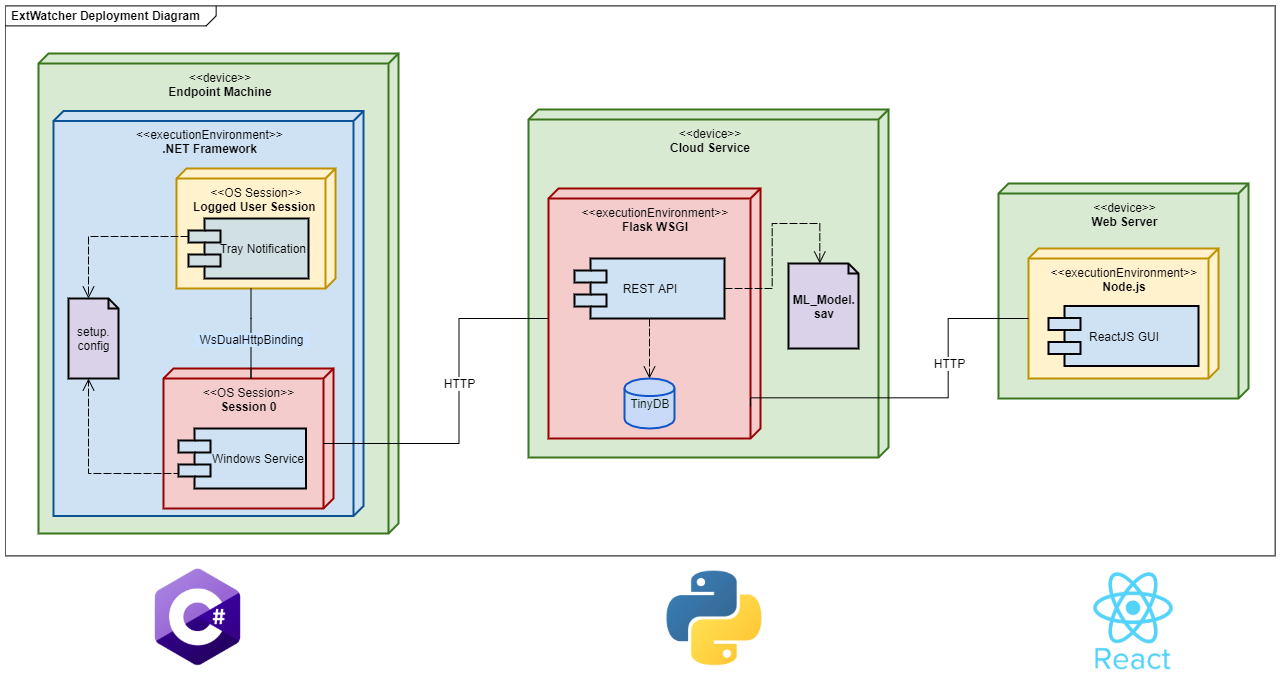
\includegraphics[scale=0.4]{figures/deployTech.png}}  
	\caption{Deployment Diagram of the application and used technologies}
	\label{deployment}
\end{figure}

The core of the entire software application is the \textit{Cloud Analyzer}, which provides the security measure against malicious PDF documents. ExtWatcher has two different, independent approaches for getting access to the Cloud Analyzer. 

\begin{itemize}
	\item The first one implies automatic file detection and requires the installation of \textit{ExtWatcher Service}, which will establish a connection through HTTP to the Cloud Analyzer and will remove instantly detected malicious files from the user's computer.
	\item The second approach is an \textit{out-of-the-box} functionality, user being able to analyze a file by accessing the Cloud Analyzer Dashboard (web graphical user interface) and entering the URL of the file. The dashboard submits the URL to the Cloud Analyzer and the later downloads the file, classifies it and sends back the verdict. This solution is fit for mobile devices, as it requires no additional installation, ExtWatcher Service being currently supported just on Windows OS.
\end{itemize}

In order to properly work, our application requires permanent Internet connection, because the core of analysis is remotely located. The advantage of this is the fact that Cloud servers are better at applying Machine Learning models for malware detection, thereby reducing the workload of personal computers. 


\section{ExtWatcher Service}
\label{section:winService}
This section will describe how the Windows Service manages to simplify the user responsability and to automate the task of detection and uploading of PDF files to our analysis engine. As previously mentioned, this is not a mandatory component, rather just a help utility for users whose computers work on Windows platform. However this tool itself integrates two separate executables (the service and the app aimed to send system notifications), each with its own configuration files. Of course, field knowledge is required in order to correctly configure this tool and to let it run errorlessly. To solve this problem and to make \textit{ExtWatcher Service} accessible for everyone, we created a Setup Installation File, which packages all the necessary files and installation information into \textit{MSI} files. The user should just launch the installer executable to get \textit{ExtWatcher Service} properly working on their computers. Under the hood, the used Windows Installer, unpackages those two applications and their configuration files, moves them to the corresponding installation folder, writes the suitable registry keys to set the \textit{Tray Notification App} to launch at the user's login, installs the service into Windows Service Manager and starts the utility right after the installation is done. 

% Before putting to disposition of the user this tool, we had to create an installer (++ winService)

\begin{figure}[H]
	\centerline{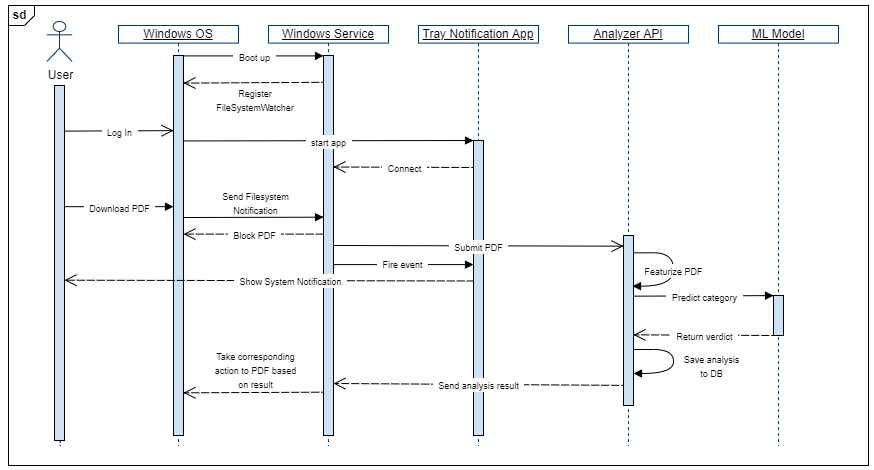
\includegraphics[scale=0.55]{figures/sequence.png}}  
	\caption{Sequence Diagram showing interaction between User, Windows Service and Cloud Analyzer}
	\label{sequence}
\end{figure}


\section{Cloud Analyzer}
\label{section:cloudApi}


\section{Dashboard Interface}
\label{section:dashboard}

\begin{figure}[H]
	\centerline{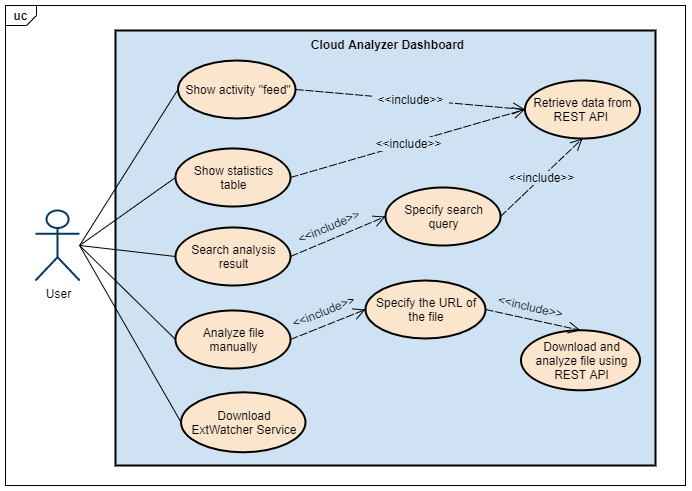
\includegraphics[scale=0.7]{figures/usecaseGUI.png}}  
	\caption{Use Case Diagram showing interaction between User and Cloud Analyzer using web GUI}
	\label{usecase}
\end{figure}